\section{Inverted Double Pendulum model} 
\begin{figure}
	\centering
	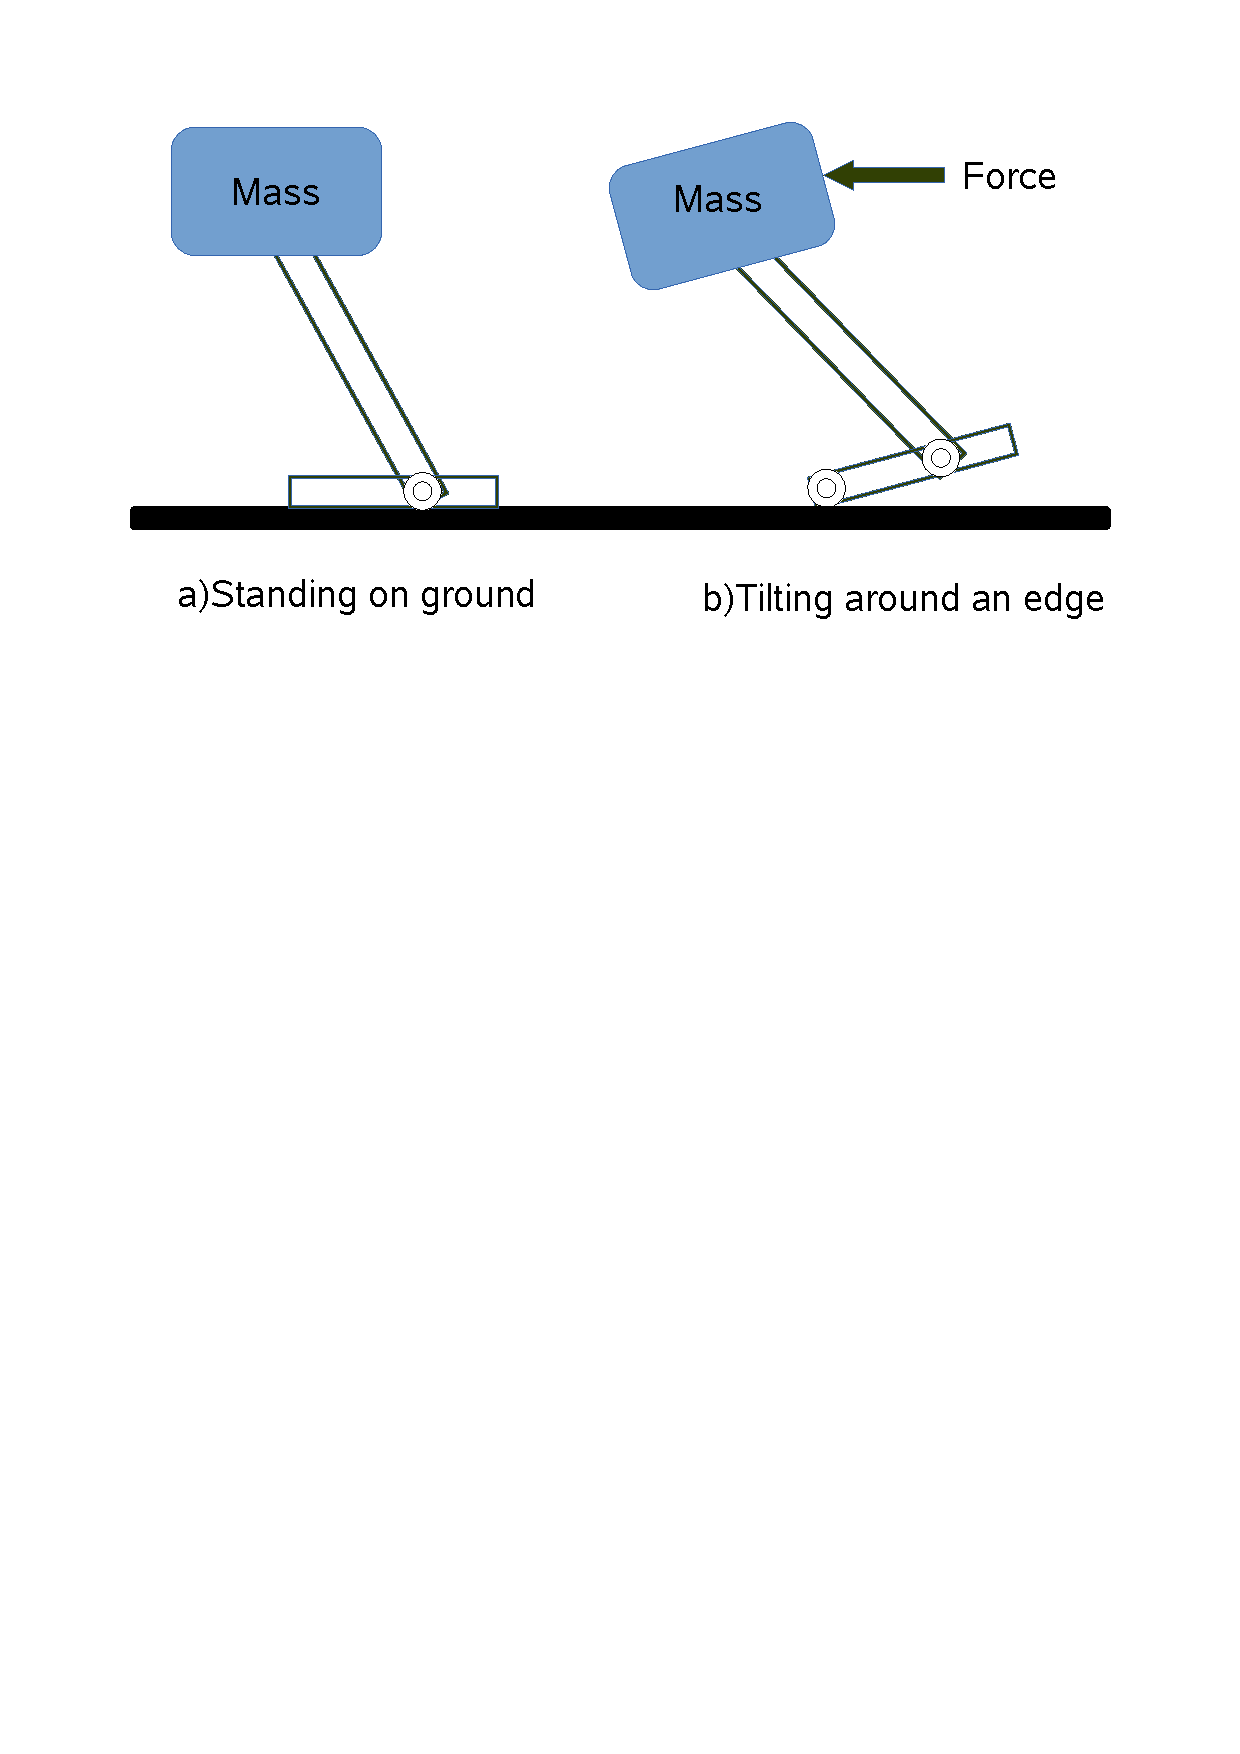
\includegraphics[trim = 0mm 160mm 0mm 30mm, scale=0.75]{Bilder/simp_uactcase.pdf}
	\caption{A simplified humanoid robot standing on one foot}
	\label{fig:idp_scene}
\end{figure}
Inorder to check the feasibility of solving the state estimation problem with the available measurements for the whole robot model, a preliminary subproblem is formulated. Since we are interested in estimating the underactuated degrees of freedom, we have to consider the senario where these underactuated degrees of freedom are action on the robot. Let us consider the senario where the robot is tilting around an edge of the foot by applying some external force as shown in Figure \ref{fig:idp_scene}.b. Figure \ref{fig:idp_scene} shows a simplified version of a humanoid robot standing on one leg. All the joints other that ankle joint of the robot are assumed to remain static(joints does not produce any motion) throughout the experiment. The kinematics of the robot is simplified to one joint on the ankle connecting the whole body with the foot as shown in \ref{fig:idp_scene}.a. The kinematics of \emph{Toro} is shown in Figure \ref{fig:toro_kin}. The mass block in the Figure \ref{fig:idp_scene} represents the inertia of upperbody. The inertia of leg is incorporated in the link connceting upperbody and foot. 

When robot is tilting around an edge of the foot as shown in Figure \ref{fig:idp_scene}.b, we assume there is an imaginary joint located at the edge of the foot around which the robot tilts. Figure \ref{fig:idp_scene}.b resmbles an inverted double pendulum in Figure \ref{fig:idp}.
\begin{figure}[H]
	\centering
	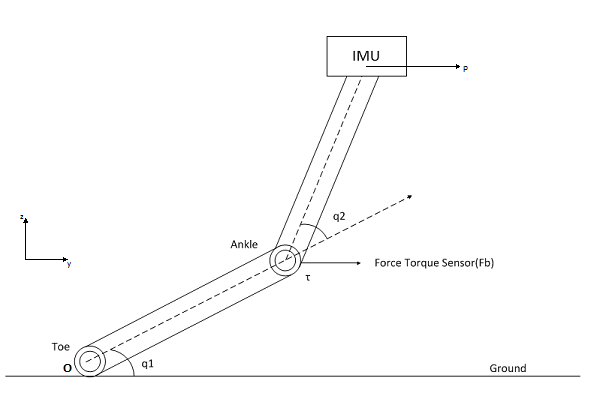
\includegraphics[scale=0.75]{Bilder/doublePendulum1.png}
	\caption{Inverted Double Pendulum}	
	\label{fig:idp}
\end{figure}
 In the inverted pendulum model the ankle joint is actuated but the toe joint is unactuated. The degrees of freedom of this model are toe and ankle. Toe is the underactuated degree of freedom whose motion parameters such as angle $q_1$ and angular velocity $\dot{q}_1$ needs to be estimated. The motion parameters of the inverted double pendulum are 
\begin{equation}
	 q = 
	\begin{pmatrix}
		q_{1}\\
		q_{2}
	\end{pmatrix}
	 \dot{q} = 
	\begin{pmatrix}
		\dot{q_{1}}\\
		\dot{q_{2}}
	\end{pmatrix},
\end{equation}
where \emph{q} is the vector of joint angles and $\dot{q}$ is the vector of joint angular velocities. The control input or torque applied to the ankle joint is $\tau$. The equation of motion of the inverted double pendulum is derived by Lagrange formulation, the generalized coordinates of the system are $q_1,q_2$ which represents the angles of the joints, $\dot{q_1},\dot{q_2}$ represent the velocities of corresponding joints as shown in figure \ref{fig:idp}.
\begin{equation}
	M(q)_{2\times2}.
	\begin{pmatrix}
		\ddot{q_{1}} \\
		\ddot{q_{2}} 
	\end{pmatrix}
	+ C(q,\dot{q})_{2\times2}.
	\begin{pmatrix}
		\dot{q_{1}} \\
		\dot{q_{2}} 
	\end{pmatrix}
	+ g(q)_{2\times 1} = \tau_{2\times 1}
\end{equation}

\begin{equation}
	\label{eq:dyn_eq}
	\begin{pmatrix}
		\ddot{q_{1}} \\
		\ddot{q_{2}} 
		\end{pmatrix}
	= M(q)^{-1} \left( -C(q,\dot{q}).\dot{q} - g(q) + \tau \right )
\end{equation}

To convert the equations into ODE's, assume 
$$ x_1 = q_1, x_2 = \dot{q_1}, x_3 = q_2, x_4 = \dot{q_2}$$
substitute the above equations into \eqref{eq:dyn_eq}. The resulting non linear dynamic equation is of form

\begin{equation}
\begin{split}\label{eq:dyn_ode}
	\dot{x}  = f(x,u),	\\
	x = 
	\begin{pmatrix}
		x_1 \\
		x_2 \\
		x_3 \\
		x_4
	\end{pmatrix}
\end{split}
\end{equation}
\eqref{eq:dyn_ode} is the model prediction equations in Kalman filter. The measurement equation is,

\begin{equation}
	y= 
	\begin{pmatrix}
		q_2\\
		\dot{q_2}\\
		a_{py}\\
		a_{pz}\\
		\omega_x\\
		Fb_y\\
		Fb_z \\
	\end{pmatrix}
\end{equation}

where,
\begin{itemize}
\item
 $q_2, \dot{q_2}$- angle and velocity of ankle joint measured by encoders
\item 
$a_{py},a_{pz}$- cartesian accelerations along \emph{x and z axis} measured by IMU(Inertial Measurement Unit)
\item
$\omega_x$ - angular acceleration around \emph{x axis} measured by gyroscope
\item
$Fb_y,Fb_z$- ground reactional froces action along \emph{ y and z axis} measured by FTS(Force Torque Sensor)
\end{itemize}
The estimated states are $$q_1, \dot{q_1}$$ are the underactuated degrees of freedom of the system.
